Los elementos presentes en la interfaz visual son los siguientes.

\paragraph{Barra lateral de configuración.}
La barra lateral permite seleccionar el número de fuentes, el modelo disponible, la base de datos, la función de pérdida y el checkpoint que se desea cargar.

\begin{figure}[H]
    \centering

    \begin{subfigure}{0.45\textwidth}
        \centering
        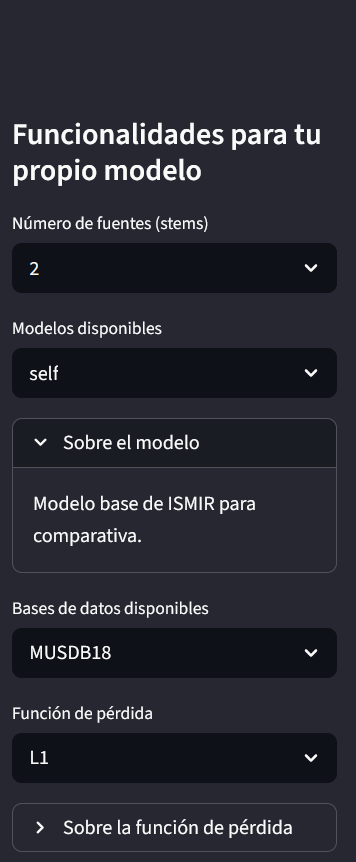
\includegraphics[width=\textwidth,height=0.55\textheight,keepaspectratio]{commons/Sidebar_GUI_1.png}
        \caption{Configuración del modelo.}
        \label{fig:sidebar-gui-1}
    \end{subfigure}
    \hfill
    \begin{subfigure}{0.45\textwidth}
        \centering
        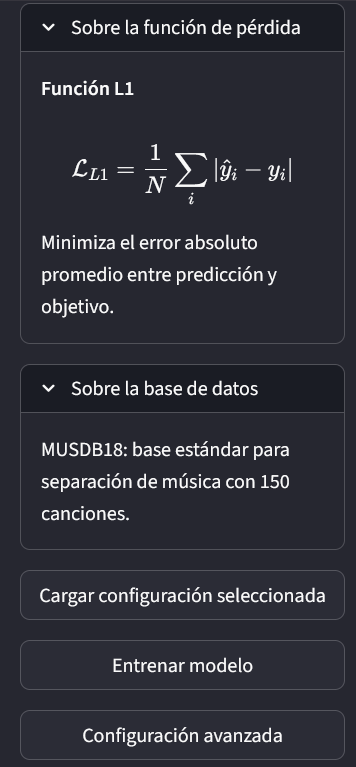
\includegraphics[width=\textwidth,height=0.55\textheight,keepaspectratio]{commons/Sidebar_GUI_2.png}
        \caption{Información auxiliar.}
        \label{fig:sidebar-gui-2}
    \end{subfigure}

    \caption{Barra lateral de configuración de la interfaz.}
    \label{fig:sidebar-gui}
\end{figure}

\FloatBarrier



\paragraph{Zona principal de carga.}
La zona principal permite subir un archivo de audio y lanzar el proceso de separación.

\begin{figure}[H]
    \centering

    \begin{subfigure}{0.45\textwidth}
        \centering
        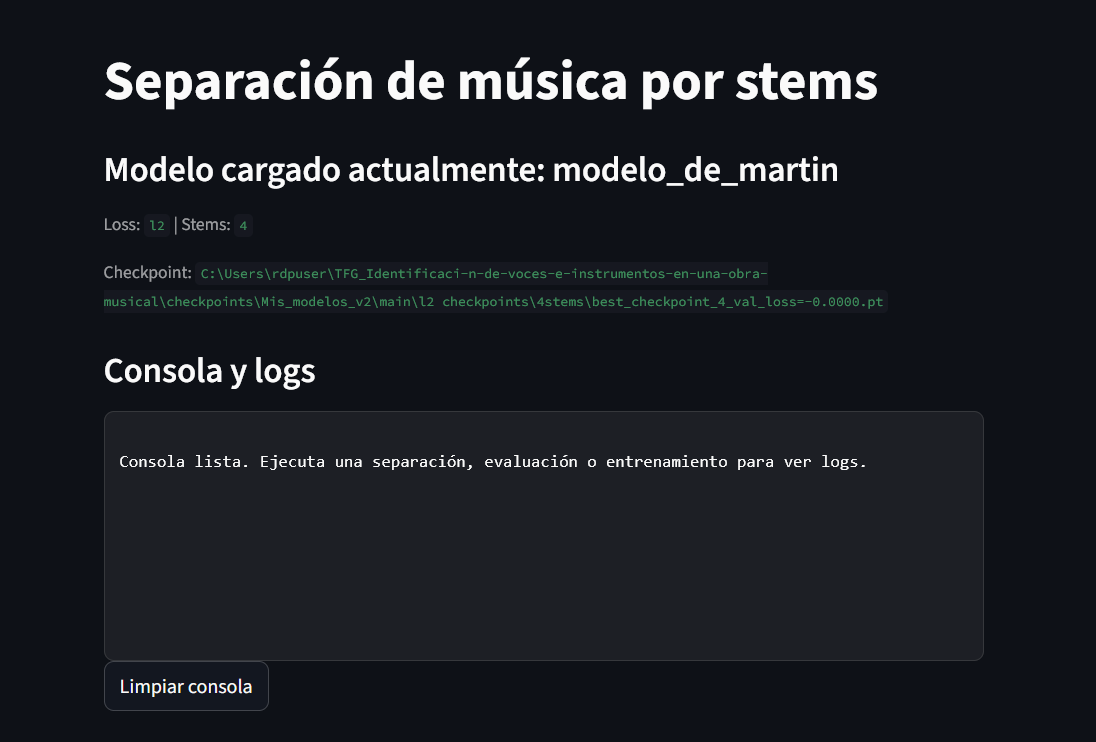
\includegraphics[width=\textwidth,height=0.55\textheight,keepaspectratio]{commons/ZonaCarga_GUI_1.png}
        \caption{Zona de carga de la GUI superior.}
        \label{fig:zona-carga-gui1}
    \end{subfigure}
    \hfill
    \begin{subfigure}{0.45\textwidth}
        \centering
        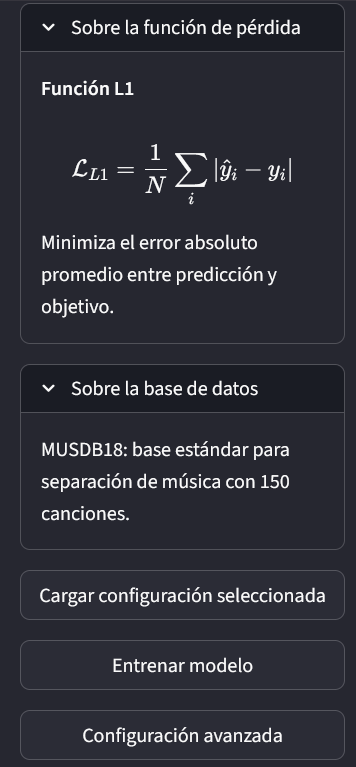
\includegraphics[width=\textwidth,height=0.55\textheight,keepaspectratio]{commons/Sidebar_GUI_2.png}
        \caption{Zona de carga de la GUI inferior}
        \label{fig:zona-carga-gui2}
    \end{subfigure}

    \caption{Zona de carga de la GUI.}
    \label{fig:zona-carga-gui}
\end{figure}

\FloatBarrier

\paragraph{Consola y logs.}
La consola muestra información sobre la ejecución del sistema, incluyendo mensajes de carga, separación, evaluación y posibles errores.

\begin{figure}[H]
    \centering
    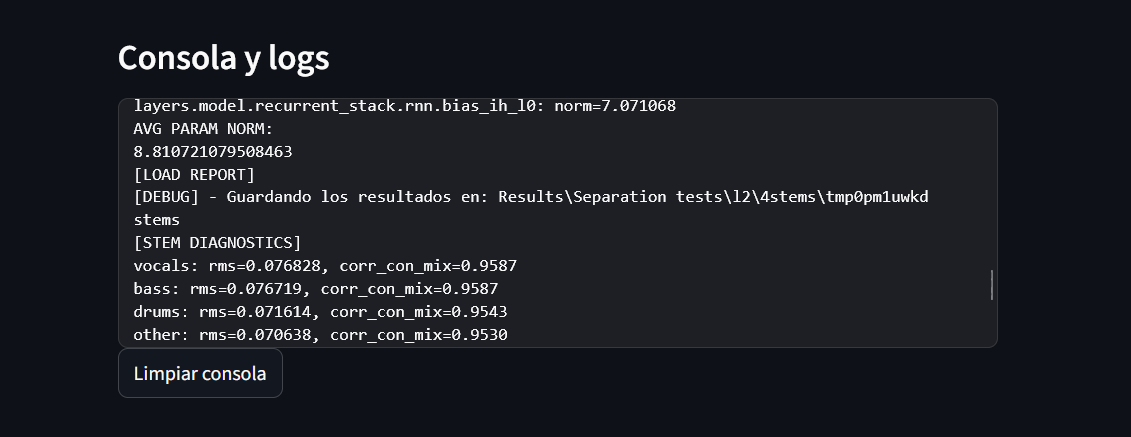
\includegraphics[width=0.75\textwidth,height=0.45\textheight,keepaspectratio]{commons/Consola_GUI_2.png}
    \caption{Consola y logs de la GUI.}
    \label{fig:consola-gui}
\end{figure}

\FloatBarrier

\paragraph{Reproductores.}
Tras la separación, la interfaz muestra reproductores de audio para la mezcla original y para cada una de las fuentes separadas.

\begin{figure}[H]
    \centering

    \begin{subfigure}{0.45\textwidth}
        \centering
        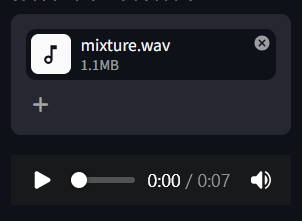
\includegraphics[width=\textwidth,height=0.16\textheight,keepaspectratio]{commons/Reproductor1_GUI.png}
        \caption{Mezcla original.}
        \label{fig:reproductor-mezcla}
    \end{subfigure}
    \hfill
    \begin{subfigure}{0.45\textwidth}
        \centering
        
\includegraphics[width=\textwidth,height=0.16\textheight,keepaspectratio]{commons/Reproductor2_GUI.png}
        \caption{Vocales.}
        \label{fig:reproductor-vocales}
    \end{subfigure}

    \vspace{0.3cm}

    \begin{subfigure}{0.45\textwidth}
        \centering
        
\includegraphics[width=\textwidth,height=0.16\textheight,keepaspectratio]{commons/Reproductor3_GUI.png}
        \caption{Bajo.}
        \label{fig:reproductor-bajo}
    \end{subfigure}
    \hfill
    \begin{subfigure}{0.45\textwidth}
        \centering
        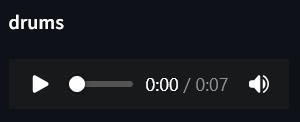
\includegraphics[width=\textwidth,height=0.16\textheight,keepaspectratio]{commons/Reproductor4_GUI.png}
        \caption{Batería.}
        \label{fig:reproductor-bateria}
    \end{subfigure}

    \vspace{0.3cm}

    \begin{subfigure}{0.45\textwidth}
        \centering
        
\includegraphics[width=\textwidth,height=0.16\textheight,keepaspectratio]{commons/Reproductor5_GUI.png}
        \caption{Otros.}
        \label{fig:reproductor-otros}
    \end{subfigure}

    \caption{Reproductores de audio de la interfaz.}
    \label{fig:reproductores-gui}
\end{figure}

\FloatBarrier

\paragraph{Gráficos.}
La interfaz también permite visualizar representaciones gráficas de las fuentes separadas, como la forma de onda y el espectrograma.

\begin{figure}[H]
    \centering
    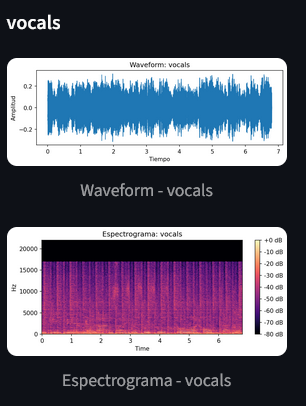
\includegraphics[width=0.85\textwidth,height=0.55\textheight,keepaspectratio]{commons/Graficos_GUI.png}
    \caption{Ejemplo de representación gráfica de la fuente vocal.}
    \label{fig:graficos-gui}
\end{figure}

\FloatBarrier

\paragraph{Botones.}
La interfaz incluye botones para lanzar la separación, evaluar el modelo y descargar los audios generados.

\begin{figure}[H]
    \centering

    \begin{subfigure}{0.45\textwidth}
        \centering
        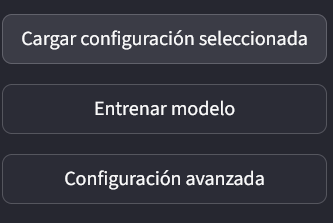
\includegraphics[width=\textwidth,height=0.16\textheight,keepaspectratio]{commons/Botones1_GUI.png}
        \caption{Botón de separación.}
        \label{fig:botones-gui-1}
    \end{subfigure}
    \hfill
    \begin{subfigure}{0.45\textwidth}
        \centering
        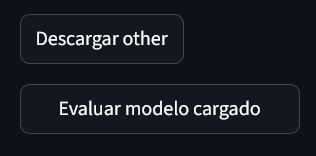
\includegraphics[width=\textwidth,height=0.16\textheight,keepaspectratio]{commons/Botones2_GUI.png}
        \caption{Botón de evaluación.}
        \label{fig:botones-gui-2}
    \end{subfigure}

    \vspace{0.3cm}

    \begin{subfigure}{0.45\textwidth}
        \centering
        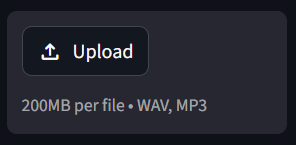
\includegraphics[width=\textwidth,height=0.16\textheight,keepaspectratio]{commons/Botones3_GUI.png}
        \caption{Botón de descarga.}
        \label{fig:botones-gui-3}
    \end{subfigure}
    \hfill
    \begin{subfigure}{0.45\textwidth}
        \centering
        
\includegraphics[width=\textwidth,height=0.16\textheight,keepaspectratio]{commons/Botones4_GUI.png}
        \caption{Botón auxiliar.}
        \label{fig:botones-gui-4}
    \end{subfigure}

    \caption{Botones principales de la interfaz.}
    \label{fig:botones-gui}
\end{figure}

\FloatBarrier